\chapter{Conception et réalisation de l'application web}

\section{Architecture logicielle}

L'application est organisée en deux parties. Le frontend est une page HTML qui contient le style CSS et le code JavaScript de la démonstration. Le backend est un service Python FastAPI chargé de l'ensemble GRU retenu et responsable du contrat d'inférence final.

Le choix de FastAPI est cohérent avec le projet, car les modèles sont entraînés avec Python et PyTorch. Le framework fournit des routes HTTP testables et un support WebSocket pour une extension future \cite{FastAPI}. Le prototype livré utilise HTTP par fenêtre afin de privilégier un contrat déterministe. Le WebSocket n'est pas présenté comme une fonctionnalité déjà validée.

\begin{figure}[ht]
\centering
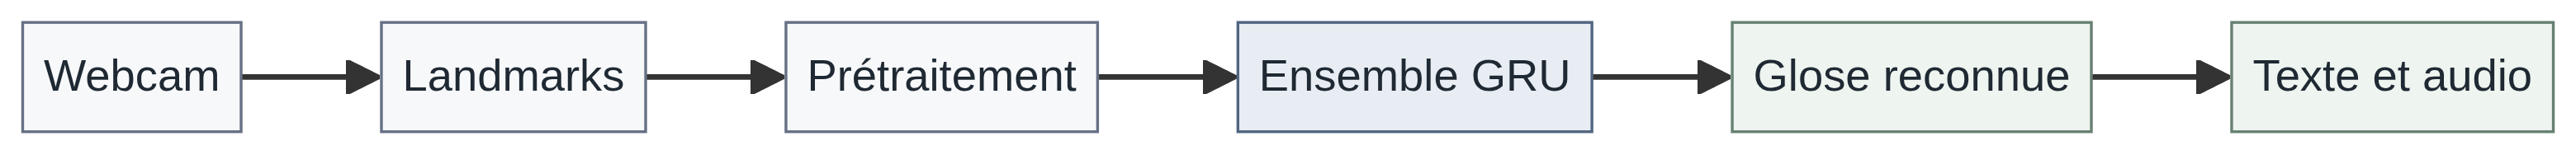
\includegraphics[width=0.90\textwidth,height=0.28\textheight,keepaspectratio]{figures/architecture_application_simple.png}
\caption{Chaîne essentielle de l'application : extraction des landmarks, prétraitement, classification par l'ensemble GRU et production d'une sortie textuelle ou audio.}
\label{fig:architecture-application}
\end{figure}

La Figure~\ref{fig:architecture-application} résume le chemin effectivement utilisé par l'interface. Les détails du contrat HTTP et les routes de comparaison sont présentés plus loin dans ce chapitre.

\section{Chaîne de données et traçabilité scientifique}

La chaîne de data science sépare les métadonnées, les séquences de landmarks, les transformations et les artefacts de modèles. Les partitions officielles et le manifeste d'intégrité sont conservés hors du dépôt public, tandis que les scripts de vérification, les configurations YAML, les métriques et les résumés sont versionnés. Le contrôle détecte les signeurs communs entre partitions, les identifiants dupliqués et les incompatibilités de forme avant l'entraînement.

Pour la phase GRU groupée, chaque exécution produit un résumé JSON, les prédictions et un checkpoint par fold. Les quinze checkpoints du modèle retenu sont conservés dans le registre des modèles. L'ensemble est agrégé par moyenne des probabilités pour l'évaluation et pour le mode actif de l'application. Le benchmark de latence distingue le temps de prédiction du modèle du temps de capture, de détection MediaPipe et de la synthèse vocale.

\section{Initialisation de la caméra et de MediaPipe}

L'utilisateur déclenche explicitement l'activation de la caméra. Le navigateur demande l'autorisation via l'API \texttt{getUserMedia}. MediaPipe Tasks Vision est ensuite chargé avec une version CDN documentée. Pose Landmarker et Hand Landmarker sont configurés en mode vidéo.

Pour chaque frame, le frontend récupère le premier résultat de pose et les résultats des mains. Une main non détectée est remplacée par 21 points nuls afin de conserver la forme de l'entrée. Cette stratégie garantit le contrat dimensionnel, mais elle ne garantit pas que l'information gestuelle soit suffisante. L'absence de mains doit donc rester visible dans l'analyse des erreurs.

\section{Capture et formation des fenêtres}

Le bouton de capture collecte 40 frames espacées d'environ 55 millisecondes. Trois fenêtres chevauchantes de 32 frames sont créées avec des débuts aux positions 0, 4 et 8. Chaque fenêtre respecte l'ordre des points défini par le contrat de prétraitement avant d'être envoyée au backend.

La méthode est volontairement cadrée. L'utilisateur réalise un signe isolé pendant la capture. Le système ne prétend pas détecter automatiquement une succession de signes dans une conversation. Cette décision réduit la complexité du démonstrateur et rend son comportement explicable.

\section{Guide d'utilisation de l'interface}

L'utilisation suit une séquence courte et déterministe. L'utilisateur clique d'abord sur « Activer la caméra » et autorise l'accès vidéo dans le navigateur. Le bouton « Analyser le signe » lance ensuite la capture d'une fenêtre de 40 frames. Le signe doit être réalisé seul, face à la caméra, dans un cadrage où les mains et le haut du corps restent visibles. Le système construit trois fenêtres chevauchantes, envoie les données à l'API et affiche les résultats classés.

La zone « Résultat » présente la meilleure glose, les trois hypothèses principales et leur score. Ce score est indicatif tant que la calibration GRU n'a pas été ajustée sur une validation hors échantillon. Le bouton « Écouter » lit le texte contrôlé associé à la prédiction ; il ne traduit pas une phrase LSFB et ne modifie pas la décision du modèle. Le bouton « Arrêter » désactive la caméra. Le bouton « Effacer » remet l'affichage à l'état initial. Une capture de l'état initial de l'interface est donnée à la Figure~\ref{fig:interface-application}.

\begin{figure}[ht]
\centering
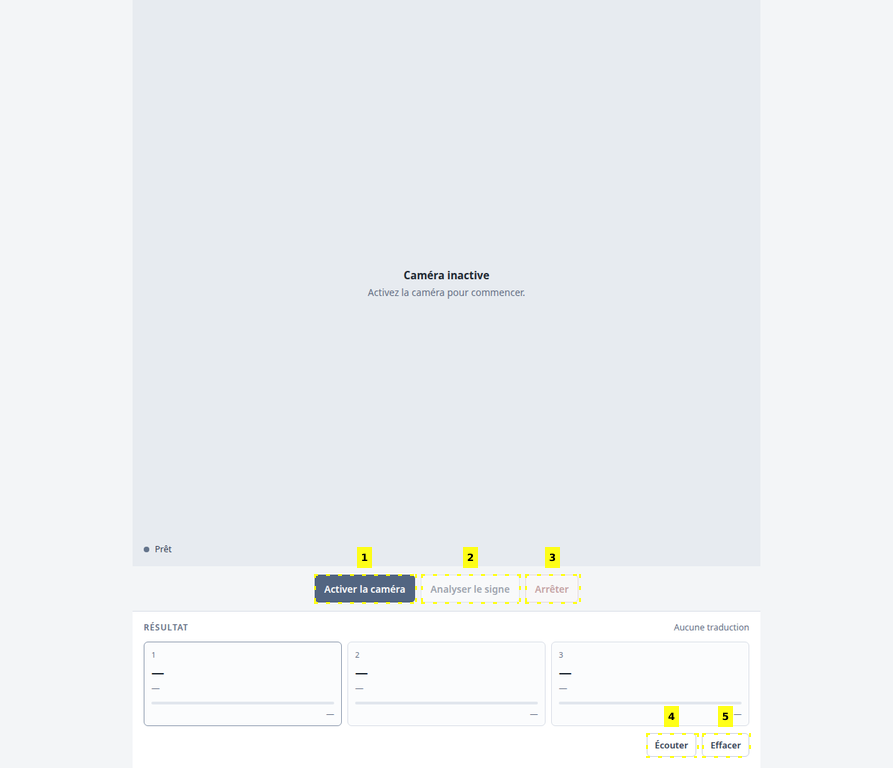
\includegraphics[width=0.62\textwidth]{figures/application_interface.png}
\caption{Interface du prototype : activation de la caméra, analyse d'un signe isolé, affichage du résultat et lecture vocale optionnelle.}
\label{fig:interface-application}
\end{figure}

Cette procédure limite les erreurs d'usage, mais elle ne constitue pas encore un protocole de traduction en visioconférence. Une application continue devra afficher l'état de la segmentation, distinguer une hypothèse temporaire d'une sortie confirmée et permettre de corriger ou d'annuler une phrase avant sa vocalisation.

\section{Contrat HTTP}

La route active \texttt{POST /predict-gru} attend un objet JSON contenant \texttt{landmarks}. La matrice reçue doit avoir exactement 32 lignes et 225 valeurs par ligne. Elle correspond aux 33 points de pose et aux 42 points de mains en trois coordonnées. L'API convertit les données en tableau NumPy, vérifie la forme et rejette les valeurs non finies.

Le backend normalise ensuite chaque frame par rapport au torse et ajoute les deux poignets relatifs au torse. La représentation interne contient 231 valeurs par frame. Les quinze GRU produisent des distributions softmax qui sont moyennées avant le classement final. La réponse conserve le score brut, le score calibré lorsqu'un artefact de calibration validé existe, la marge entre les deux premières classes et l'accord des quinze réseaux.

La réponse contient la glose prédite, sa confiance, les trois meilleurs résultats, le temps d'inférence, la version du modèle et la représentation utilisée. Elle indique aussi \texttt{confidence\_calibrated}, \texttt{raw\_confidence}, \texttt{margin}, \texttt{ensemble\_agreement}, \texttt{accepted} et \texttt{rejection\_reason}. Tant qu'une calibration apprise sur validation groupée n'est pas installée, \texttt{accepted} vaut \texttt{null} et aucun rejet scientifique n'est déclaré. Les routes \texttt{/health} et \texttt{/model-info} servent respectivement au diagnostic et à l'inspection des métadonnées de l'ensemble actif.

Le Tableau~\ref{tab:contrats-http} récapitule les routes actives, historiques et de comparaison ainsi que leurs formes d'entrée.

\begin{table}[ht]
\centering
\small
\caption{Contrats HTTP du prototype et statut de chaque route.}
\label{tab:contrats-http}
\begin{tabular}{p{4.3cm}p{2.5cm}p{9.4cm}}
\hline
Route & Entrée principale & Fonction et statut \\
\hline
\texttt{/health} & Aucune & État du service, modèle actif et nombre de checkpoints \\
\texttt{/model-info} & Aucune & Métadonnées de l'ensemble GRU retenu actif \\
\texttt{/candidate-info} & Aucune & Métadonnées du RF historique conservé pour le repli \\
\texttt{/predict-gru} & \texttt{[32,225]} & Route finale de l'interface web \\
\texttt{/predict} & \texttt{[32,225]} & Route baseline conservée pour les tests \\
\texttt{/predict-candidate} & \texttt{[32,126]} & Route RF historique conservée pour comparaison \\
\hline
\end{tabular}
\end{table}

La route \texttt{/predict-gru} est la seule route de prédiction utilisée par l'interface finale. Les autres routes restent accessibles pour la traçabilité, la comparaison et le retour arrière, mais ne sont pas proposées comme choix à l'utilisateur.

\section{Stabilisation de la décision}

Le classement et le rejet sont deux décisions distinctes. La future règle de rejet combinera le score calibré, la marge top-1--top-2 et l'accord des quinze réseaux. Les seuils seront appris sur une validation groupée par signeur en optimisant le risque à couverture fixée ; ils ne seront pas choisis à partir du test officiel. Dans l'état courant, la calibration n'est pas encore installée, l'interface affiche le top-3 et le statut « score non calibré », et la vocalisation reste désactivée sous le seuil d'interface historique de 55 pour cent.

La stabilisation agit au niveau de l'interface. Elle ne modifie pas les paramètres du classifieur et ne transforme pas une mauvaise prédiction en bonne prédiction. Elle constitue une règle de décision applicative et non une amélioration mesurée du modèle. Une calibration future ne changera pas le classement top-1 ; elle rendra seulement le niveau de confiance et le rejet plus interprétables.

\section{Génération du texte et synthèse vocale}

Une table JavaScript associe chaque classe à un texte français contrôlé. Le texte est affiché après validation de la stabilité. La Web Speech API crée automatiquement une utterance vocale pour la meilleure prédiction stable, c'est-à-dire la classe retenue par le modèle lorsque le seuil de confiance applicatif est atteint \cite{WebSpeech}. Un bouton secondaire permet uniquement de répéter le dernier résultat. La logique annule une vocalisation précédente avant d'en lancer une nouvelle et mémorise la dernière décision prononcée afin d'éviter les répétitions.

Le modèle produit une classe de glose. La table de sortie lui associe un texte contrôlé. Le navigateur produit ensuite le son. La qualité de la voix dépend du navigateur et des voix installées ; elle doit être documentée comme une propriété de la couche de présentation et non comme une performance de reconnaissance LSFB.

Un mode expérimental peut enchaîner des segments causaux et conserver une liste de gloses. Cette liste constitue une étape vers la transcription visuelle de séquences, mais elle ne doit pas être appelée transcription continue validée sans corpus comportant des séquences annotées, des frontières temporelles et une mesure par distance d'édition.

\section{Gestion des erreurs et sécurité du contrat}

L'API refuse les entrées de forme incorrecte et les valeurs non finies. Au démarrage, elle vérifie la correspondance entre les classes, le nombre de caractéristiques et les métadonnées de configuration. Ces contrôles empêchent de charger silencieusement un modèle incompatible avec le frontend.

Les tests automatisés couvrent le healthcheck, les métadonnées, une prédiction GRU valide, une forme incorrecte et une valeur non finie. Le test de robustesse sur 5\,957 séquences confirme également le rejet de trois payloads invalides par le code HTTP 422. Ces contrôles ne remplacent pas un test navigateur, mais ils garantissent le contrat backend minimal.

\section{Migration intermédiaire vers le Random Forest mains seules}

Une migration intermédiaire vers \texttt{wrist\_scaled} a d'abord été réalisée pour réduire la dimension de l'entrée et vérifier la cohérence entre le frontend et un modèle RF. Le frontend conservait alors les 42 points des deux mains, appliquait le même centrage et la même échelle que le script d'entraînement et utilisait \texttt{/predict-candidate} avec une entrée \texttt{[32,126]}. L'ancien contrat pose--mains \texttt{[32,225]} et la baseline historique ont été conservés pour les tests et le retour arrière.

Cette étape RF a été utile comme champion intermédiaire. Elle a toutefois été dépassée par l'évaluation groupée des modèles GRU, qui a apporté un gain sur le test officiel dans le protocole final. La migration RF reste documentée afin de rendre la chronologie reproductible.

\section{Bascule finale vers l'ensemble GRU retenu}

La bascule finale a remplacé le contrat actif par \texttt{/predict-gru}. Le frontend transmet les landmarks de pose et des mains sous la forme \texttt{[32,225]}. Le backend applique la normalisation par le torse, ajoute les poignets relatifs et exécute les quinze checkpoints du modèle retenu. Les artefacts, leurs manifestes et les tests sont conservés dans GitHub.

La décision d'activer la GRU repose sur deux niveaux de preuve. La comparaison finale sur le test officiel donne une accuracy de 82,31 pour cent et un macro-F1 de 0,8153. Le test API indépendant de l'implémentation hors ligne, réalisé sur les 5\,957 mêmes séquences, reproduit ces métriques. La GRU est donc le modèle actif dans le périmètre étudié, tandis que le RF reste une solution de comparaison et de repli.

\section{Tests d'inférence et mesure de latence}

Un benchmark synthétique de la route \texttt{/predict-gru} a mesuré une moyenne HTTP de 68,19 millisecondes sur 10 appels. Le test de robustesse sur le split officiel a mesuré une moyenne de 63,59 millisecondes, une médiane de 59,57 millisecondes, un P95 de 86,79 millisecondes et un P99 de 109,41 millisecondes par séquence.

Ces chiffres caractérisent le trajet HTTP et l'inférence GRU sur des landmarks déjà extraits. Ils n'incluent pas l'acquisition de la caméra, l'extraction MediaPipe, la consolidation complète des fenêtres ni la synthèse vocale. La mesure de la chaîne complète nécessite un protocole de capture dédié sur un poste équipé.

\section{Portée de la notion de temps réel}

L'application actuelle fonctionne par fenêtres : elle capture 40 images, construit trois fenêtres de 32 frames, attend la fin de la capture, puis envoie les fenêtres au backend et consolide les réponses. Le prototype fournit ainsi une interaction rapide après une capture, mais il ne réalise pas une traduction continue frame par frame.

Le système actuel fonctionne comme une reconnaissance interactive de gloses LSFB isolées par fenêtres, avec sortie textuelle contrôlée et synthèse vocale optionnelle après capture. La reconnaissance continue demanderait une acquisition en continu, une segmentation causale validée, une mesure de latence de bout en bout, un corpus de séquences annotées et une évaluation sur vidéo réelle.

\section{Conclusion du chapitre}

Ce chapitre a décrit l'architecture finale du prototype. La capture, l'extraction des landmarks, le prétraitement GRU, l'inférence de l'ensemble configuration GRU retenue, la stabilisation et la synthèse vocale sont séparés par des contrats vérifiables. L'application fournit une reconnaissance interactive de gloses isolées ; le RF est conservé pour le repli, tandis que la traduction continue reste hors du périmètre démontré.

Le chapitre suivant discute les performances, les erreurs résiduelles, les limites de l'évaluation API et les perspectives nécessaires pour passer d'une reconnaissance isolée à une chaîne webcam complète.
